
%% ----------------------------------------------------------------
%% Thesis.tex -- MAIN FILE (the one that you compile with LaTeX)
%% ---------------------------------------------------------------- 

% Set up the document
\documentclass[a4paper, 11pt, twoside]{Thesis}  % Use the "Thesis" style, based on the ECS Thesis style by Steve Gunn
\graphicspath{{Figures/}}  % Location of the graphics files (set up for graphics to be in PDF format)

% Include any extra LaTeX packages required
\usepackage[square, numbers, comma, sort&compress]{natbib}  % Use the "Natbib" style for the references in the Bibliography
\usepackage{verbatim}  % Needed for the "comment" environment to make LaTeX comments
\usepackage{vector}  % Allows "\bvec{}" and "\buvec{}" for "blackboard" style bold vectors in maths
\usepackage{tabulary}
\usepackage{tikz}
\usepackage{gantt}
\usepackage{rotating}
\usepackage{pdflscape}
\usepackage{Sweave}
\usepackage{graphics}
\usepackage{float}
\usepackage{hyperref}
\usepackage{placeins}


\newcommand{\includecode}[2][C]{\lstinputlisting[caption=$2, escapechar=, style=custom$1]{$2}}

\lstdefinestyle{customc}{
  belowcaptionskip=1\baselineskip,
  breaklines=true,
  frame=L,
  xleftmargin=\parindent,
  language=C,
  showstringspaces=false,
  basicstyle=\footnotesize\ttfamily,
  keywordstyle=\bfseries\color{green!40!black},
  commentstyle=\itshape\color{purple!40!black},
  identifierstyle=\color{blue},
  stringstyle=\color{orange},
}

\lstdefinestyle{customasm}{
  belowcaptionskip=1\baselineskip,
  frame=L,
  xleftmargin=\parindent,
  language=[x86masm]Assembler,
  basicstyle=\footnotesize\ttfamily,
  commentstyle=\itshape\color{purple!40!black},
}

\lstset{escapechar=@,style=customc}



\hypersetup{urlcolor=blue, colorlinks=true}  % Colours hyperlinks in blue, but this can be distracting if there are many links.

%% ----------------------------------------------------------------
\begin{document}
\frontmatter      % Begin Roman style (i, ii, iii, iv...) page numbering
% Set up the Title Page
\title  {Delta Printer Project Report}
\authors  {\texorpdfstring
            {\href{mailto:k9brown@students.latrobe.edu.au}{Keith Brown}}
            {Author Name}}
\addresses  {\groupname\\\deptname\\\univname}  % Do not change this here, instead these must be set in the "Thesis.cls" file, please look through it instead
\date       {\today}
\subject    {}
\keywords   {}

\maketitle


%% ----------------------------------------------------------------


\setstretch{1.3}  % It is better to have smaller font and larger line spacing than the other way round

% Define the page headers using the FancyHdr package and set up for one-sided printing
\fancyhead{}  % Clears all page headers and footers
\rhead{\thepage}  % Sets the right side header to show the page number
\lhead{}  % Clears the left side page header

\pagestyle{fancy}  % Finally, use the "fancy" page style to implement the FancyHdr headers

%% ----------------------------------------------------------------

% Declaration Page required for the Thesis, your institution may give you a different text to place here
\Declaration{

\addtocontents{toc}{\vspace{1em}}  % Add a gap in the Contents, for aesthetics

\begin{figure}[htbp]
\centering
        \resizebox{\textwidth}{!}{\includegraphics{./EE_Statement_of_Authorship.pdf}}
 \end{figure}
}
\clearpage  % Declaration ended, now start a new page


% The Abstract Page
\addtotoc{Abstract}  % Add the "Abstract" page entry to the Contents
\abstract{
\addtocontents{toc}{\vspace{1em}}  % Add a gap in the Contents, for aesthetics

This document describes the design and development of an inexpensive 3D printer. The project is developed for the final year engineering project at La Trobe University by Keith Brown.

The printer will be in the form of a delta machine. The intention is to reduce the number of components and utilise cheaper hardware while still achieving a fast accurate print. The electronics will not be a direct derivative of current implementations. Experimentation with alternative architecture will be trialled with the goal of delivering a more computational capable system.

An introduction into 3D Printing and its concepts, advantages and issues is outlined. The commercial viability for both commercial and consumer markets is described. An analysis of both the structure and the systems inverse kinematic equations are included. Considerations regarding fluid motion is outlined. Hardware diagrams and descriptions follow. The electronic and software systems are discussed in detail. Testing procedures and associated results are also examined. Finally, project management tasks are reviewed.

 


}

\clearpage  % Abstract ended, start a new page

%% ----------------------------------------------------------------


\setstretch{1.3}  % Reset the line-spacing to 1.3 for body text (if it has changed)

% The Acknowledgements page, for thanking everyone
\acknowledgements{
\addtocontents{toc}{\vspace{1em}}  % Add a gap in the Contents, for aesthetics
I would like to share my sincere gratitude to Dr Robert Ross, my primary supervisor whom has given me so much creative control. Robert has provided constant assistance. He also has bestowed me with his precious technical expertise. Adam Console my co-supervisor, has helped steer this project in the right direction on numerous occasions. It was Adam that suggested the delta machine design. His diverse knowledge is irreplaceable.

The RepRap community has paved the way for projects like this. There is a wealth of freely available information on their website and forums. I hope that I will be able to express my appreciation by giving something back to the open source community.

I would like to personally thank everyone who has supported me. I have discussed this project with many of my friends and family, who have contributed with valuable support and feedback.


}
\clearpage  % End of the Acknowledgements
%% ----------------------------------------------------------------

\pagestyle{fancy}  %The page style headers have been "empty" all this time, now use the "fancy" headers as defined before to bring them back


%% ----------------------------------------------------------------
\lhead{\emph{Contents}}  % Set the left side page header to "Contents"
\tableofcontents  % Write out the Table of Contents

%% ----------------------------------------------------------------
\lhead{\emph{List of Figures}}  % Set the left side page header to "List if Figures"
\listoffigures  % Write out the List of Figures

%% ----------------------------------------------------------------
\lhead{\emph{List of Tables}}  % Set the left side page header to "List of Tables"
\listoftables  % Write out the List of Tables

\mainmatter
\pagestyle{fancy}

\chapter{Introduction}
\label{Introduction}
\lhead{ \emph{Introduction}}

3D Printers have received a lot of media attention recently. Additive manufacturing has been around for at least 30 years \cite{1, 2}. However, in the last five years popularity has increased dramatically due to the availability of much cheaper entry level machines. It is now possible for the general public to purchase pre-assembled printers at a similar cost as a personal computer.

There will always be innovation and dangers associated with a new technology. We already have prime examples of both aspects; At a 2011 TED talk, Dr Anthony Atala presented a human kidney prototype that his team had printed \cite{3}. Late 2012 Cody Wilson uploaded a video to Youtube that showed himself firing a gun mostly composed of 3D printed parts \cite{4}.

The environment will benefit from this new way of producing products. Firstly, plastic items can be recycled and reused to create new, more useful items. This not only reduces costs but it also eliminates transportation of new items. They no longer need to be imported and transported all over the country, they can just be downloaded.

Whilst companies like Objet and Stratasys produce printers for the commercial sector, it is hobbyist style printers that have spread awareness of such technology. The Reprap foundation has produced numerous models under the GPL licence. Their main goal is to produce an affordable device that can self replicate. All of the designs are available to download and print. Makerbot Industries is a comercial operation that was born from an open source community.

Online services such as Shapeways provides 3D printing services. This allows their customers to receive a higher quality print without investing in expensive hardware. CAD design community sites have also been very popular such as 'thingiverse.com'. There are over 30,000 free designs including a key-chain fob, mobile phone case, model radial engine and even 3D printer parts and upgrades.

\section{3D printing methods}

Additive manufacturing is the process of constructing a three-dimensional object by depositing material in discrete layers. Conversely, traditional machining methods are subtractive; material is removed to expose the desired object. This printer utilises an additive method as it produces fine plastic layers to build an object. There are many different approaches of additive manufacturing. The main four methods are outlined in the following paragraphs.

Fused deposition modelling or FDM is the method of extruding thermoplastics in layers.
 This project is considered to use an FDM method as it extrudes fine plastic layers to build an object. The printer deposits plastic material by melting it through a hot extruder. The extruder resembles a metal funnel that takes solid plastic and produces liquid plastic out of a small hole. The liquid plastic can be fused to previously deposited material. The machine must physically move the extruder around an area, while placing plastic where it is required. This process is repeated layer by layer to achieve a three-dimensional object. The technology was invented by S. Scott in 1980 \cite{2}.

Selective laser sintering or SLS is a technique that allows either metal, plastic, ceramic and glass powder to be fused together with a powerful laser. The laser targets cross-sections, selectively fusing a fine layer of powder to the object. Once a layer has been complete, a fresh layer of powder is dusted over the object and the process repeats. The left over material acts as a support for the object being manufactured. After the procedure has finished, the excess powder can be removed and used for the next print. The process is slow, producing porous but strong results.

Stereolithography or SLA is the method of using an ultraviolet light to cure a photopolymer. The printing platform sits in a vat of liquid resin. The light targets a cross-section of the desired object and the exposed resin will solidify. Once the layer has completed, the platform will move down allowing for another layer to be added to the model. SLA produces accurate results but is a very slow process. SLA has received a lot of attention recently as the method has been adopted by a handful of young start ups. It offers a much greater result compared to the current generation of FDM printers. However the hardware and resin is very expensive.

Laminated object manufacturing or LOM is another rapid prototyping method. It uses a laser or a knife to cut out layers from an adhesive-coated material. The layer is then heated and pressed onto the previous layers. A new sheet of material is rolled in place and the process repeats. This method can be relatively cheap as readily available material such as paper can be used.

Each process is managed by a technique called '\textit{computer numerical control}' or CNC. This method is essentially computer controlled automation. Three-dimensional models are developed using '\textit{Computer aided design}' or CAD. These CAD models are processed to produce CNC commands known as G-code. The G-codes are instructions that tell the  machine how to produce the CAD model.
\section{FDM Articulation implementations}

A Cartesian Gantry structure is the most common implementation. It consists of a linear actuator for each axis of freedom. The horizontal plane generally has a sturdy rail that a bridge is mounted on, this rail permits motion in the x direction. A carriage is mounted to a rail that connects the bridge together. The carriage can move along this rail and therefore permits motion in the y direction. Lastly the carriage has a tool that is capable of actuating in and out in the z direction.

The Gantry system is a well tested framework and is industry standard. It can be found in many applications from small desktop CNC machines to huge container cranes. While the frame is very strong, each linear actuator is dependent on another. The bridge actuator has to be the strongest as it must provide enough force to move the bridge, carriage and tool. This becomes an issue for fast moving applications as the momentum will be relatively large.

The Delta robot has three vertical rails placed in the formation of an equilateral triangle. Each linear actuator moves in the same direction and has kinetic linkages that connect each carriage to a central platform. This platform can be positioned by placing each carriage at a certain height. This is an improvement over the Gantry setup because each actuator shares the load equally. It is capable of faster speeds because there is less load on the tool end.
\section{FDM accuracy and materials}

Currently, leading consumer 3D printers can produce objects with layers heights of 0.1 millimetres. Such an accurate print will generally take around five hours for a medium sized print. Pricing for a mostly pre-assembled unit is around USD\textdollar 2,200.

Currently there are two main types of plastics readily available for FDM printing. Firstly Acrylonitrile Butadiene Styrene or ABS is a strong material. It is a oil based plastic that can be melted and extruded at a temperature of approximately 105 \textdegree C. It is fairly cheap at \textdollar 40 a Kg. It does contract slightly as it cools.

Polylactic Acid or PLA is another alternative that can be used for FDM printing. It is marginally less expensive then ABS. While being more brittle then ABS it does not contract as much. PLA is a biodegradable polymer and actually is produced by corn starch. Because of it's lower melting point it is not ideal for applications related to heat.
\section{Proposed Solution}

The delta machine design has been adopted for this project. Recently the Rostock project has spawned many derivatives, most achieving cheaper construction over the last generation of reprap printers. Delta machines have been used for many applications including; pick and placers, packaging and production line sorters.

Its simplicity helps reduce hardware costs. But the biggest advantage is the machines speed and accuracy. If the central platform is kept light, fast acceleration can be maintained. This permits the machine to perform in a sporadic manner while maintaining an accurate position.

The electronics system will not be a derivative of current implementations. I will experiment with different architectures with the goal of producing a much cheaper but fully capable system. The components will be made modular to allow for a high level of customisation. This helps to keep the main-board costs low but still permits additional more expensive upgrades such as a Ethernet add on.
\section{Commercial Viability}

This old technology is becoming established in a new market. While it becomes more accessible, new opportunities begin to emerge and intern, increases demand. Prices are decreasing, materials are becoming more accessible and there is an increasing amount of printable designs being uploaded to the Internet. The later attributes the most positive influence to the 3D printing market. This makes an old product more valuable.

\begin{figure}[H]
\centering%
\includegraphics{fig/intro/growth.pdf}
\caption{Growth of CAD designs on thingiverse.com \cite{6}}
\label{fig:growth.pdf}
\end{figure}
It is clear that this market is expanding at a promising rate. Furthermore because there is such a diverse range of neighbouring markets that will benefit from this technology, it is likely that it will be supported by commercial demand alone. Applications for 3D printing have yet to be completely discovered, the boundaries are always being pushed by innovators. It is apparent that a very successful industry has been created.


\subsection{Commercial Market}

3D printing can help many different businesses. For example; Product designers can produce prototypes within a few hours, prosthetics can be made for a person more frequently and engineers can produce custom parts easily. It is important to note that even if a 3D printer existed in every home, there are still many skills that can't be replaced by automation. Downloading a generalised product will never replace a professionally crafted custom version. 3D printing just streamlines the development cycle and promotes rapid growth.

Rapid prototyping reduces development costs and creates new opportunities. It is possible that we will see a rise in hardware start-ups similar to the influx of software start-ups we have seen recently. It may be more feasible for a young company to attempt entering into established markets with little overhead.

\subsection{Consumer Market}

There is a number of reasons why an individual might desire a 3D printer. It may help reduce our consumption rate by allowing us to easily repair broken household items. While it is unlikely for the average person to need a miniature factory, it is ideal for hackers, hobbyists, artists and craftsmen

Currently, the largest consumer market for 3D printing falls inside the open source community. Although intellectual property is freely shared, support and labour is very valuable. These customers are generally open to early adoption of new technology. The network of passionate, diversely skilled customers strive to improve the current designs and collaboratively innovate the CNC scene.
\chapter{Structure and Inverse Kinematics }
\label{Structure and Inverse Kinematics }
\lhead{ \emph{Structure and Inverse Kinematics }}

The hardware design will be in the form of a delta machine. These devices can perform fast accurate tasks as the light-weight print head is capable of quick acceleration. This design has been adopted from a current reprap project \cite{5}. The delta machine will use less parts then a traditional Cartesian machine.

For a detailed overview of this projects design please refer to the Design Document

\section{Structure}

A delta machine consists of a number of kinetic chains that meet at a central platform. This platform can be moved by actuating the pivots connected to the main structure. The platform is kept parallel to the floor during motion. Figure \ref{fig:structure_diagram.svg} represents a simple two armed delta machine. The two-dimensional diagram helps to illustrate the important lengths and vectors. After we have analysed a two dimensional machine we will apply these concepts to three-dimensions.

\begin{figure}[H]
\centering%
\includegraphics{fig/structure_positioning/structure_diagram.pdf}
\caption{Structure Diagram}
\label{fig:structure_diagram.svg}
\end{figure}
\begin{table}[!h]
\centering
\begin{tabulary}{\textwidth}{LL}
\hline\hline
 $D$  &  Distance from actuator to origin                       \\
 $L$  &  Vertical length of the frame                           \\
 $a$  &  Height of the actuator pivot point from the origin     \\
 $h$  &  Length of the kinetic linkage                          \\
 $r$  &  Radius of the platform                                 \\
 $p$  &  Position of the extruder tip or centre of the platform \\
 $O$  &  Origin of the system                                   \\
 $x$  &  Horizontal vector                                      \\
 $y$  &  Vertical vector                                        \\
 $z$  &  Depth vector                                           \\
\hline
\\
\end{tabulary}
\caption{	List of vectors}
\label{1}
\end{table}



The following assumptions are made to help define the system:
\begin{itemize}
\item  Platform and linkages must stay within the frame's outer rails.
\item  Linkages are not restricted in any way, they may swivel on their joins in any direction.
\item  The platform can not move down past the base.
\item  Linkages are restricted to the rail's length.
\item  Linkages can not stretch or contract.
\end{itemize}
\section{Simple one dimension position}

Lets consider one dimension to begin with, Figure 1 illustrates the movement of three key points; the platform and the left and right linear actuators. We can see that if the linkages are the same length as the vertical distance, the platform is capable of reaching any position along the $x$ axis.



Also, it can be seen that a vertical actuator requires an equal amount of travel to permit full movement. It is important to note that the platform is considered a point source in this example. Practically this is not the case as we will require a place to mount tools.

For a desired position of $p(x)$, we need to derive where to place linear actuators. Take fig. \ref{fig:structure_simple.svg} below, lets derive the equations that will translate a desired $x$ into $a_1$ and $a_2$. 

\begin{figure}[H]
\centering%
\includegraphics{fig/structure_positioning/structure_simple.pdf}
\caption{Simple one dimension parameters}
\label{fig:structure_simple.svg}
\end{figure}

Firstly, lets derive relationship between $x$ and $a_1$:
$$ (1)\  h^2 = a^{2}_{1} + b^{2}_{1} $$
$$  \Leftrightarrow  a_{1} = \sqrt{ h^2 - b^{2}_{1} }$$
$$ (2)\  b_1 = x - (-D)$$
$$ \Leftrightarrow\  b_1 = x + D$$
substituting (1) into (2) gives
$$ a_1(x) = \sqrt{ h^2 - ( x + D )^2 }$$
Now, lets find the relationship between $x$ and $a_2$:
$$ (3)\  h^2 = a^{2}_{2} + b^{2}_{2}$$
$$  \Leftrightarrow  a_{2} = \sqrt{ h^2 - b^{2}_{2} }$$
$$ (4)\  b_2 = x - D$$
finally, substituting (4) into (3)
$$ a_2(x) = \sqrt{ h^2 - (x - D)^2 } $$
\section{Platform}

We now need to consider what happens to the linkages when they are offset by the platforms width.



By adding extra length to the horizontal component, we have decreased the horizontal outer bounds of the system. The smaller the platform the more room we are able to travel. It should also be noted that the larger the platform, the less vertical travel is required for the actuators.

The Platform reduces the $b_1$ and $b_2$ term in our position equation by $r$. We now have:
$$ a_1(x) = \sqrt{ h^2 - (x + D - r)^2 }$$
$$ a_2(x) = \sqrt{ h^2 - (x - D + r)^2 } $$
\section{Vertical travel constraints}

We can also reduce the vertical travel required by reducing the linkages length. This intern reduces the available printing area. However, this can be used to our advantage. For example if we needed to restrict the horizontal bounds so that the platform can't physically interfere with the belt drive that runs alongside the vertical rails.


\section{Two dimensional position in the vertical plane}

Now we are able to examine how we may add a vertical component to the system. From the last sections we discovered that the length required for the vertical actuators is the equal the linkages length. In this example, we have created a square printable area of $(2D)^2$. This is possible as the rails are twice the length of the linkages length or $L = 2(2D)$. 



Introducing the $z$ component directly adds to the $a_1$ and $a_2$ terms. The position equations are amended as:

$$ a_1(x) = \sqrt{ h^2 - (x + D - r)^2 } \color{red}{ + z}$$
$$ a_2(x) = \sqrt{ h^2 - (x - D + r)^2 } \color{red}{ + z}$$
\section{Two dimensional position in the horizontal plane}

Now its time to examine how adding a third actuator allows for two dimensional movement in the horizontal plane. Figure \ref{fig:top-view_diagram.svg} is a top-down view of our system. The actuators are placed in a equilateral triangle formation to distribute the load evenly. The position of the platform can be altered by changing the lengths of the linkages horizontal component, the $b$ term. Remember, this is not stretching the linkages, it is merely displacing length between the horizontal and vertical component - the hypotenuse remains the same. By looking straight down into the system, only the $b$ vectors are visible, the carriages on the rails or the $a$ term is  directed in/out of the page.

The coordinates system has been aligned with the actuators to help simplify the problem. The origin is placed at the centre of the print bed. Please note that the print bed is represented as a circle with its radius equal to the minimum distance from the origin to the frame. 

To control the platforms position we must modify the carriages vertical position $a$. However, the horizontal plane position is completely dependent on $b$. We have already established the relationship between $a$ and $b$, and that is $a = \sqrt{ h^2 - b^2}$. We now need to develop the relationship between $b$ and the position ($x,y)$.

Each actuator will have its own equation for calculating its $b$ term. This is because they are not placed uniformly around the coordinates system even though they are equally apart. Firstly, the general rule for calculating $b$ as a function of the platforms position:
$$b_n(x,y) = |\overrightarrow{R_n P(x,y)}|$$ Where R is the position vector of the target actuator and P is the position vector of the platform.

\begin{figure}[H]
\centering%
\includegraphics{fig/structure_positioning/top-view_diagram.pdf}
\caption{Top view components}
\label{fig:top-view_diagram.svg}
\end{figure}
Figure \ref{fig:top-view_diagram.svg} illustrates that this problem can be solved by a simple application of Pythagoras' theorem again.

Top actuator:
$$d_1(x) =  x$$
$$e_1(y) =  y - D$$
$$b_1(x,y) = \sqrt{d_1^2 + e_1^2}$$
$$b_1(x,y) = \sqrt{ x^2 + (y - D )^2}$$
Bottom left actuator:
$$d_2(x) = x - (-d\sqrt{3}/2)$$
$$e_2(y) = y - (-d/2)$$
$$b_2(x,y) = \sqrt{ ( x + {d\sqrt(3)\over 2})^2 + ( y + {d\over 2})^2   } $$
Bottom right actuator:
$$d_3(x) = x - D\sqrt{3}/2$$
$$e_3(y) = y - (-D/2)$$
$$b_3(x,y) = \sqrt{ ( x - {D\sqrt(3)\over 2})^2 + ( y + {D\over 2})^2   } $$
\section{Platform in the horizontal plane}



Adding a platform with a radius of $r$ just offsets our $x$ and $y$ components. The amended equations are:

$$b_1(x,y) = \sqrt{ x^2 + (y + {\color{red}{r}} - D )^2}$$
$$b_2(x,y) = \sqrt{ ( x {\color{red}{- {r\sqrt(3)\over 2}}}  + {d\sqrt(3)\over 2})^2 + ( y {\color{red}{- {r\over 2}}} + {d\over 2})^2   } $$
$$b_3(x,y) = \sqrt{ ( x {\color{red}{+ {r\sqrt(3)\over 2}}} - {D\sqrt(3)\over 2})^2 + ( y {\color{red}{- {r\over 2}}} + {D\over 2})^2   } $$
\section{Three dimensional positioning }

Both horizontal and vertical components have been explained and now can be combined into one system. To implement a three dimensional system, we simply need to replace our $b_n$ variable in the vertical plane equation with the horizontal plane equations. The result is:

$$a_1(x,y,z) = \sqrt{ h^2 - |{ x^2 + (y + r - D )^2}| }$$
$$a_2(x,y,z) = \sqrt{ h^2 - |{ ( x - {r\sqrt(3)\over 2} + {d\sqrt(3)\over 2})^2 + ( y - {r\over 2} + {d\over 2})^2 }| } $$
$$a_3(x,y,z) = \sqrt{ h^2 -  |{( x + {r\sqrt(3)\over 2} - {D\sqrt(3)\over 2})^2 + ( y - {r\over 2} + {D\over 2})^2   }| } $$
\section{Constraints}

\subsection{Printing Bed}
A design assumption was made at the beginning of this section; The platform can not be positioned outside of the frame. To force this rule to apply, we must set the linkages length equal to the minimum distance from a rail to a side of the frame. The maximum length required is a line straight down the y axis from the rail to the frame which is equal to ${\sqrt{3}\over 2}D$. If we swing the platform around, pushing it to the maximum radius that this length permits, we see that the path is not actually a circle but a rounded triangle. The light blue path in fig. \ref{fig:top-view-angle_diagram.svg} is the maximum positions. Such an unusual path is typically not needed, so we will simplify our problem by using a circular print bed.


To allow for a platform, we must subtract its radius from each of the linkages length. So, our rule for $h$ is:
$$h = {\sqrt{3}\over 2}D - r $$

\subsection{Universal Joint Angle Range}


\begin{figure}[H]
\centering%
\includegraphics[width=100mm]{fig/structure_positioning/top-view-angle_diagram.pdf}
\caption{Universal joint angle horizontal range}
\label{fig:top-view-angle_diagram.svg}
\end{figure}
The universal joints that will pivot to allow full movement will need to be capable of a certain range. This can be calculated exactly with:

$$ \theta = 60 - 2 \arctan{({  { {2 - \sqrt 3 }\over 2} r  \over  {1\over 2} D   } )} $$

Practically, we can simplify the problem by aiming for $60^{\circ}$ in the horizontal direction and $90^{\circ}$ in the vertical direction.
\chapter{Motion}
\label{Motion}
\lhead{ \emph{Motion}}

\section{Path Tracing}

Once a three dimensional object has been split up into two dimensional layers, the extruder head must trace the outlines of each layer. Once a layer has been traced, the z component moves a step down and the extruder will trace the next layer. The process repeats until all layers have been extruded leaving a fully formed three dimensional object.

To move the extruder in a desired direction, we must calculate the distance and direction that each actuator must travel. This can be done by subtracting actuator heights from the last position with the heights of the next move. This gives us three vectors describing the distance and direction. The next step is to translate these distances into corresponding speeds. To move in a straight line, each actuator must complete their respective distances at the same time. 

So to calculate how fast each actuator must move, we first start with:

$$ speed = displacement / \Delta time $$

So we can see that keeping the time constant for all three actuators, only displacement affects speed. Actually speed is directly proportional to the distance that needs to be travelled. 

But how long is an acceptable time to travel? This is quite simple once the maximum speed is determined. The actuator with the largest displacement should travel at maximum speed.

$$ \Delta time = displacement / MAX(speed) $$

Now we simply substitute the same $\Delta time$ for the other actuators. Now we have proportional motion! 
\section{Acceleration}

Acceleration is required to ensure smooth motion is maintained. Smooth motion is essential for reaching high speeds and also to minimise a stepper motor skipping a step. The rate of acceleration can be written as a function of current and next frames momentum.  We are only concerned with the momentum of the actuator carriages, not the momentum of the platform.

$$ P = mv $$
where $P$ is momentum,
$m$ is mass,
$v$ is velocity.
So to decrease momentum around sharp bends, we must reduce the speed of the actuator.

Once the system has been constructed, we will need to run tests to work out the maximum speed that we should attempt to accelerate to. Jerk is the derivative of acceleration. It can be thought of as how fast can we accelerate? This also will need to be thoroughly tested. But we can write it as a variable so that we can later substitute different values.


The acceleration algorithm is as follows:

\begin{itemize}
\item  calculate the closest change in direction for any actuator
\item  if change is less then 100 steps decrease speed by A
\item  if change is greater then 100 increase speed by A
\item  if maximum speed has been reached do nothing.
\item  repeat next step
\end{itemize}


This creates a smooth linear acceleration. We could also implement more detailed patterns that perhaps use a quadratic to reach the maximum speed sooner.
\chapter{Hardware}
\label{Hardware}
\lhead{ \emph{Hardware}}

Now that we understand the physical constraints we can start to design the physical system. Firstly, lets reiterate over some of the main objectives that relate to this section:

\begin{itemize}
\item  Kit like assembly
\item  Cheap hardware
\item  Solid and sturdy construction
\end{itemize}

\section{Frame}

The first iteration of design utilised aluminium to build the framework. It was selected due its strength and the modularity it offered during the prototyping stage.

\begin{figure}[H]
\centering%
\includegraphics[width=40mm]{fig/hardware/system30_img.JPG}
\caption{System30 Beam}
\label{fig:system30_img.JPG}
\end{figure}
Positives
\begin{itemize}
\item  Very strong in any direction
\item  Simple mounting and joining
\item  Reusable
\item  Easy to modify / tune
\end{itemize}

Negatives
\begin{itemize}
\item  Relatively expensive at \textdollar 25 per meter
\item  Requires special cutting tools
\item  Hard to source
\end{itemize}

However during the initial design, it was decided that the carriage designs would be too complex which would violate one of our design goals. The very cheap and easily obtained 8mm threaded and smooth rods were used instead. This way we can use LM8UU linear bearings instead of investing a lot of time in hardware design.

\begin{figure}[H]
\centering%
\includegraphics[width=60mm]{fig/hardware/8mm_lm8uu.jpg}
\caption{8mm round bar and LM8UU Linear bearings}
\label{fig:8mm_lm8uu.jpg}
\end{figure}Positives
\begin{itemize}
\item  \textdollar 3.3 per meter for stainless steel round bar
\item  \textdollar 0.90 per meter for 8mm threaded rod.
\item  \textdollar 0.75 per unit for LM8UU linear bearings.
\item  Easy to obtain from metal fabricators or general hardware stores
\item  Can cut with a hacksaw or angle grinder
\end{itemize}

Negatives
\begin{itemize}
\item  Flexes in the horizontal direction
\end{itemize}


\begin{figure}[H]
\centering%
\includegraphics[width=40mm]{fig/hardware/frame.pdf}
\caption{Early Sktech Of Frame Design}
\label{fig:frame.svg}
\end{figure}
The frame will have a small enclosed area for the electronics and power supply. The printer bed is mounted on top of the case. There is a beam on the top level that intersects the face in half. This is primarily for a place to mount the plastic feeder but also serves as a structural support beam.

We will need to know how much material to order. There is 4 equilateral triangles with side lengths of $D$  and there are 4 rails that need to be of $D$. 
$$M_{threaded} = 3(4D) + 2(D\sqrt{3}) $$
$$M_{smooth} = 3(2*2D)  $$
To minimise waste, $D$ needs to be a multiple of the purchased material's length.  To further reduce waste, the purchased length should be close to a whole number.



\section{Frame Brackets}

\subsection{Bottom Level}

\begin{figure}[H]
\centering%
\includegraphics[width=80mm]{fig/hardware/bracket_bottom.png}
\caption{Frame Bottom Bracket}
\label{fig:bracket_bottom.png}
\end{figure}
This design was an attempt to reduce the part count by incorporating as much functionality into a single piece. Firstly, the 4 holes on the outer perimeter are for threaded rods that will connect to other brackets that will form the base of the equilateral triangle. The clamps in the centre hold on to the parallel smooth rod that form the linear actuator and that attach to the top brackets. The screws that put pressure on the clamps also couple the stepper motor to the bracket.

\subsection{Top Level}
\begin{figure}[H]
\centering%
\includegraphics[width=80mm]{fig/hardware/bracket_top.png}
\caption{Frame Top Bracket}
\label{fig:bracket_top.png}
\end{figure}
A symmetrical design allows us to recycle many similar parts. Comparing the bottom bracket to the top bracket we can see that the only difference is the recessed enclosure for a 608zz bearing. They are recessed  so that the bearings do not fall out during operation.

\section{Platform}


\begin{figure}[H]
\centering%
\includegraphics[width=80mm]{fig/hardware/platform.png}
\caption{Platform}
\label{fig:platform.png}
\end{figure}
The platform is simply a base to mount a tool to while connecting each linkage to a linear actuator. In the Centre there are three holes that stand offs attach to. The outer holes are where the ball bearings are seated.

\section{Linkages}

The linkages are made up of 4mm threaded rod cut to a specific length. The rod is currently attached to 10mm Traxxas Rod Ends to allow movement between the carriages and the platform. These are originally for model RC car and are reasonably priced for their quality.

\begin{figure}[H]
\centering%
\includegraphics[width=80mm]{fig/hardware/trac5347.jpg}
\caption{Traxxas Rod Ends w/Hollow Balls Large}
\label{fig:trac5347.jpg}
\end{figure}\section{Linear Actuators}

\subsection{Carriage}
\begin{figure}[H]
\centering%
\includegraphics[width=80mm]{fig/hardware/carriage.png}
\caption{Carriage}
\label{fig:carriage.png}
\end{figure}
The outer holes with the relief cut mount LM8UU linear bearings. They are placed in with M3 screws clamping them into place tightly. A belt runs up through the centre with a small plate pressing against the frame fixing the belt to the carriage. The horizontal bore are where the linkages mount to. A 30mm M3 bolt holds the rod ends in place.

\subsection{Belt Drive}
I have opted to use GT-2 belt with 2mm pitch. The GT-2 grooves are far finer then the original T2.5 x 5mm Belt. Finer grooves will help produce smoother motion. The belts are made from neoprene rubber and have  fibreglass reinforcing running through them.

\subsection{Pulley and idlers}
The gears that match the belt were also printed. They were generated using the OpenScad \href{http://www.thingiverse.com/thing:16627}{Parametric pulley library} by user \href{http://www.thingiverse.com/droftarts/designs}{'droftart'} from Thingiverse. This is a great library, it offers great flexibility. The tooth profiles themselves are actually generated from the original manufactures DXF images.

The Pulley attaches to the stepper motor in the reverse orientation so that the lock nut is easily accessible and so the belt lines up with the top bracket. The idler is sandwiched between two 608zz bearings in the top bracket.

The gears must be perfect. It took a few trail runs before a straight tooth profile was obtained. The best printing settings are obviously fine, 0.25mm layer heights and full infill. Care must be taken when leveling the printing bed, it is actually better to have the bed slightly further down from the extruder so the higher layers do not clump together and warp during printing. 

\begin{figure}[H]
\centering%
\includegraphics[width=80mm]{fig/hardware/gear.png}
\caption{Gear and idler}
\label{fig:gear.png}
\end{figure}
\subsection{Motors}
Standard common Nema 17 stepper motors have been used in this design. They feature 1.8 deg/step ands are capable at driving a single coil with up to 2.5A. They can be obtained for \textdollar 15 each.

They can provide plenty of torque and are typically powered with 12 to 24 volts. The Steppers that were purchased are a normal bipolar configuration with four leads. 

\begin{figure}[H]
\centering%
\includegraphics[width=80mm]{fig/hardware/Nema_17_Stepper_Motor.jpg}
\caption{Nema 17 Stepper Motor}
\label{fig:Nema_17_Stepper_Motor.jpg}
\end{figure}

\section{Tool End}

\subsection{Plotter}

\begin{figure}[H]
\centering%
\includegraphics[width=80mm]{fig/hardware/tool_end/plotter.png}
\caption{Plotter Attachment}
\label{fig:plotter.png}
\end{figure}
Before 3D printing, I wanted to be able to test and perfect the performance of the machine. A plotter attachment was developed so that the paths generated could be analysed. A barrel was designed to hold a normal ball point pen. The pen is cut in half and the spring is reversed so that it is always pushing against the target surface. Horizontal screws fix the pen in place and the vertical screws attach the plotter to the platform.

The metal tip of the pen has a wire soldered, this is to be used when automating the height calibration. The base is currently made from a copper plate which is kept at ground. The pen tip is pulled high with a 10K resistor, so if the tip meets the base the tip will be pulled low. We can detect the voltage change with our microcontroller. 

\begin{figure}[H]
\centering%
\includegraphics[width=80mm]{fig/hardware/tool_end/homed.jpg}
\caption{Plotter Homed}
\label{fig:homed.jpg}
\end{figure}\subsection{FDM Tool}

\subsubsection{Extruder}

The extruder that will be used is the inexpensive common J-head extruder. It features a PEEK nylon tube with ventilation holes to help reduce heat transfer up into the platform. The hot end is a block of aluminium for a light weight tool. A 100K themistor is embed in the block along side a 5.6 ohm, 1\%, 5W resistor which is used as a heating element.

\begin{figure}[H]
\centering%
\includegraphics[width=80mm]{fig/hardware/tool_end/jhead.jpg}
\caption{J-head Extruder}
\label{fig:jhead.jpg}
\end{figure}
A clamp setup was developed to attach the extruder to the platform. Stand offs are used to space the extruder away from the platform so that the maximum printing depth is available. A tube clamp is fixed on top of the extruder for use with a Bowden feeder system (explained in the following section).

\begin{figure}[H]
\centering%
\includegraphics[width=80mm]{fig/hardware/tool_end/extruder.png}
\caption{Extruder Attachment}
\label{fig:extruder.png}
\end{figure}

\subsubsection{Bowden Filament Feeder}

A Bowden Filament feeder is a design that aims to reduce the weight on the tool end. The principle is by reducing the mass, we can increase the acceleration. By shifting a heavy direct drive stepper motor off the platform and fixing it onto a stationary point, we have greatly reduced the moving mass.

Instead of feeding filament directly into the extruder, it is fed first through a strong PTFE tube. The tube itself does not flex much so the force eventually builds up enough that the filament must push through the least resistances and that becomes the hot end.

A fair amount of force is required to push the filament through a length of pipe and through the extruder. This is why I have selected to use a geared configuration to increase my motors torque. A Herringbone gear arrangement is used as transfers power more evenly because more then two teeth mesh together at one time. They are also easily manufactured with 3D printing. The gears were borrowed from \href{http://www.thingiverse.com/thing:104615}{robo\_kid22 on Thingiverse}.


\begin{figure}[H]
\centering%
\includegraphics[width=80mm]{fig/hardware/tool_end/feeder.png}
\caption{Bowden Filament Feeder}
\label{fig:feeder.png}
\end{figure}
The design features a door like mechanism that is spring loaded to apply pressure on the filament. It pushes a bearing against a bolt that has had a rough surface machined into it. This provides good traction between the filament and does not slip. The filament is then fed directly into the tube which is coupled to the moving platform. The feeder is mounted on the top of the frame with a spool of plastic along side it.


\chapter{Electronic Systems}
\label{Electronic Systems}
\lhead{ \emph{Electronic Systems}}

\section{Methodology}

The first iteration of electronics were designed around the goal of modularity. While it offered the needed flexibility during the prototyping stage, a few shortcomings forced a redesign. It featured small daughter boards that vertically plugged into a mainboard. Exposing a SPI bus as ports that could accept any type of add on provides a possible upgrade path in the event of a necessary addition. 

\begin{figure}[H]
\centering%
\includegraphics{fig/electronics/modular.jpg}
\caption{First iteration of electronics}
\label{fig:modular.jpg}
\end{figure}
Unfortunately this configuration was too flimsy. Stepper drivers were damaged during testing. There is a lot of manual work required to assemble such a design and would not be practical for a final product.

The second revision was designed to be a simple low-cost single board solution. Instead of being a complete standalone product, this version is designed to leverage of a host computer. No external memory is used so a computer must constantly feed G-Code commands during a print. 

\begin{figure}[H]
\centering%
\includegraphics{fig/electronics/electronics.jpg}
\caption{Second revision}
\label{fig:electronics.jpg}
\end{figure}

One of the main goals of revision two was to be cross compatible with the exiting community firmware. The most compatible firmware is \href{http://github.com/Traumflug/Teacup_Firmware}{'Teacup'} . Furthermore, any software that I develop should be cross compatible with existing hardware such as RAMPS.


\section{High Level Diagram}

Efficient circuit board design was achieved by using the hierarchy model. The numerous duplicated parts can be abstracted and then replicated the desired amount. This also makes managing a large project far easier. This also speeds up circuit board development since that we only need to lay tracks for a single component and then propagate them to similar 'rooms'.

Examining the top level diagram, we can see that the each of the three actuators utilise two components; the stepper driver and a end stop. The extruder component contains one stepper driver and also heater circuity, while the heated bed only holds a heater. 


\begin{figure}[H]
\centering%
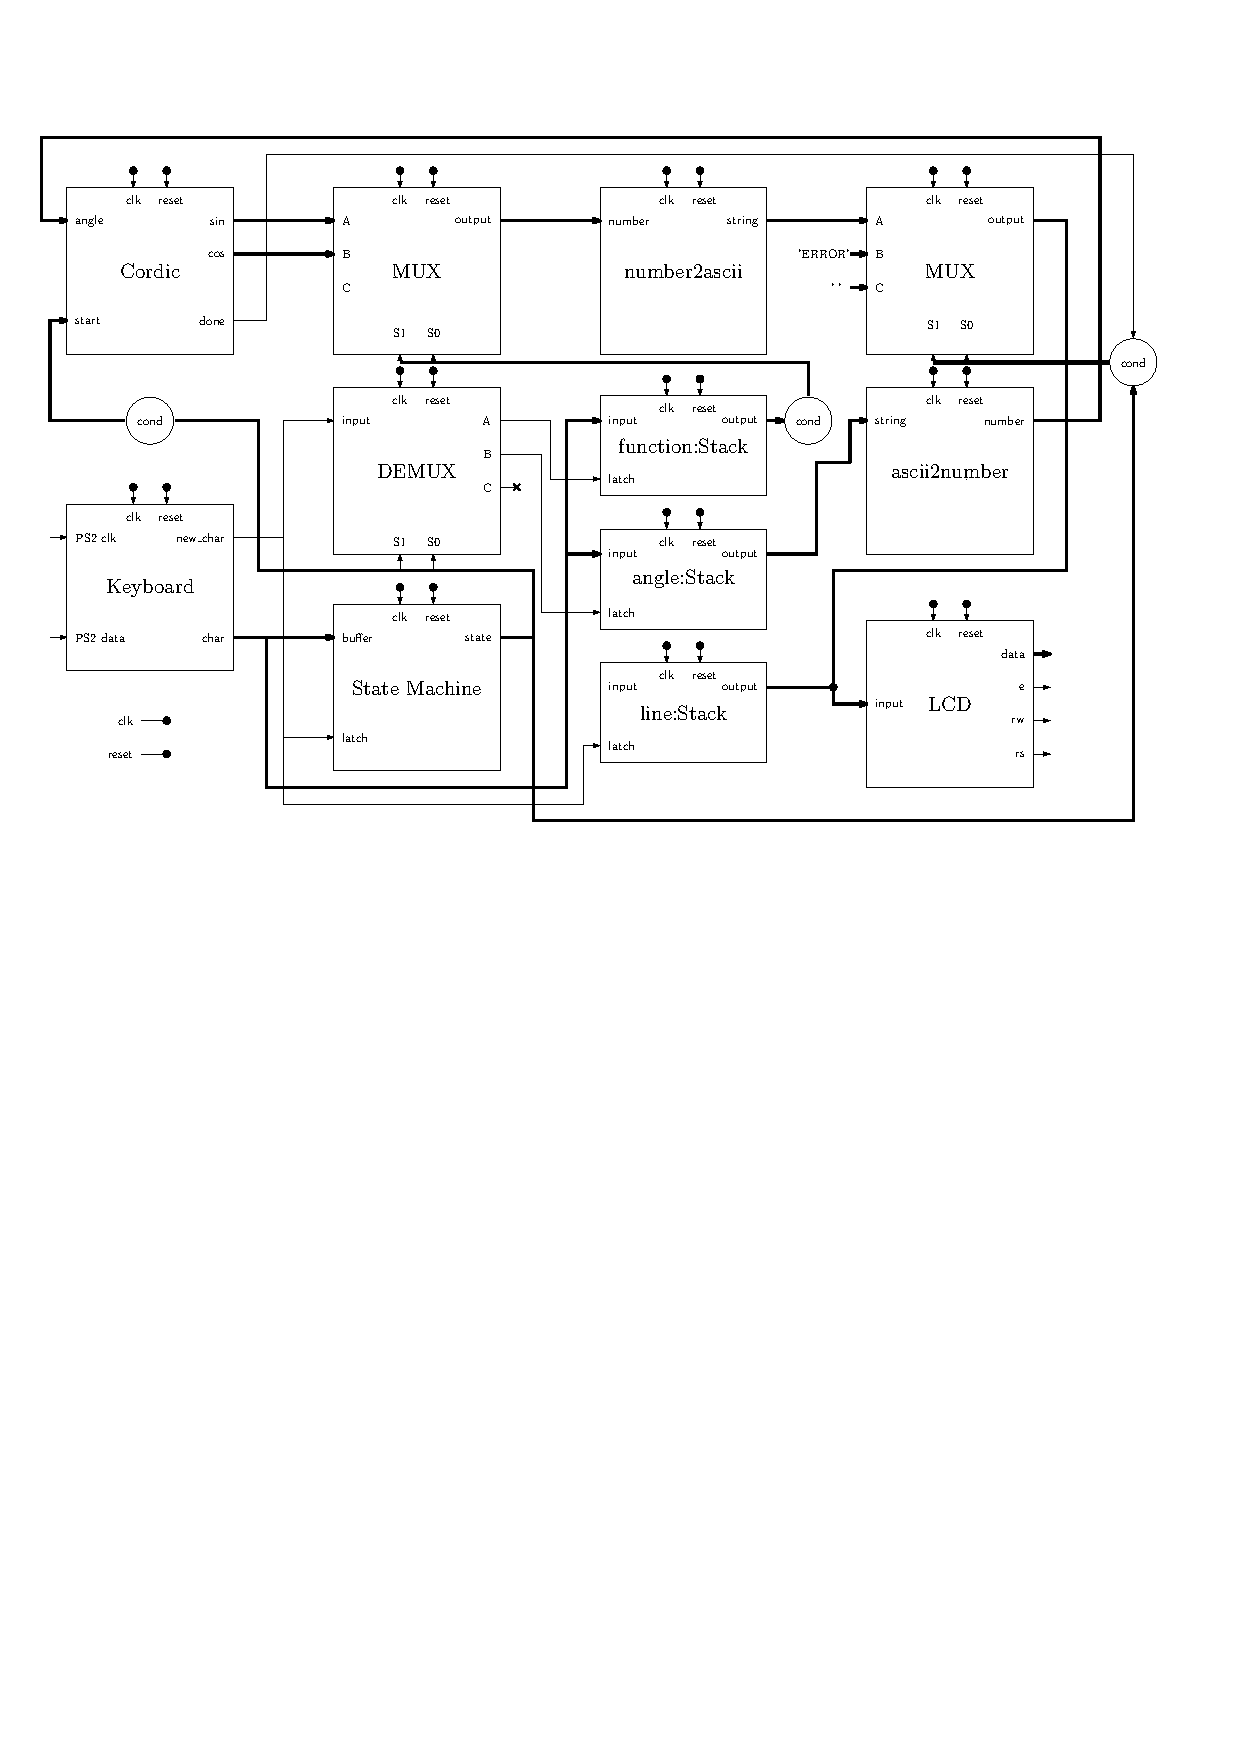
\includegraphics{fig/electronics/top_level.png}
\caption{Top Level Diagram}
\label{fig:top_level.png}
\end{figure}\section{Microcontroller}

The Microcontroller that has been selected is an Atmel 8-bit ATmega644. It was selected due to its low cost, small footprint and compatibility with existing firmware. The large ATmega family also allows for an upgrade path if required. It can be clocked up to 20MHz however I am using 10AU model which has a maximum of 10Mhz. The 10AU is available in single quantities at \textdollar 4 compared to the 20Mhz at \textdollar 11.

The package includes 64 Kbytes of flash memory. It has 44 pins with a total of 32 GPIO available. No USB communication is integrated so a USB to UART chip is required. The physical package selected was a TQFP so that it can be easily soldered with a standard soldering iron.


\section{Motor Drivers}

TI DRV8825 integrated motor drivers were selected to drive the stepper motors. They can be configured to drive a single bipolar stepper motor at 2.5A with up to 1/32 microstepping. They do not require many external passive components. They feature a useful error signal pin that goes high in the event of over current or heating issues. A heat sink should provide adequate heat dissipation.
\section{Communication}

An FTDI FT220X USB to UART converter is used for communication between the host computer and the printer. It runs at a baud rate of 38400, however burst commands can be sent due the internal FILO buffer included in the integrated circuit. A micro USB header was selected so that common android phone cables can be used.
\section{Heating elements}

A powerful MOSFET is used to push large current through a small resistor. This produces heat. The heat can be monitored with a robust thermistor. A PID loop will smoothly and accurately maintain a specific temperature. Two heat ports are available; one for the extruder and one a heated bed.
\section{Sensory input}

To determine where the platform is in the work space, the printer must first 'home'. This is the act of synchronising the memory coordinates with the actual physical coordinates. It can be achieved by firstly, moving all actuators to the top of the rails. A sensor triggers when the carriage has reached the very top so that the motor can stop. Once all carriages have reached the very top, the platform is sent back down towards the base. This is done by moving all carriages at the same time. Another sensor detects when the tool end has just touched the platform signalling the end of travel. Once this occurs, all software variables $(x,y,z)$ can be set to 0 indicating a homed tool.

The top 'end stops' have been implemented with Photo-interrupter modules. These have a IR LED that shine a beam of light into a photo-transistor. If something gets in the way of this beam, the transistor will switch off. In this case, a small height adjustable square plate attached to the carriage breaks the IR beam. See figure x

\begin{figure}[H]
\centering%
\includegraphics{fig/electronics/endstop.jpg}
\caption{Photo-interrupter}
\label{fig:endstop.jpg}
\end{figure}

The bottom plate contact is currently triggered when the tool end tip touches the grounded plate. The tip is pulled high through a 10K resistor and this level is monitored by a transistor. When a contact is made the transistor's base is forced low signalling the end of travel has occurred. While this produces great results, it is not practical in the long run once we move away from a copper plate. It would be nice to print on a fibreglass board so it can be removed. Fibreglass is not conductive so the current method will not work.

A possible alternative is to use a switch that can be retracted during print. This possible adds a servo to the tool end increasing weight. Another alternative would be to use a IR range finding system. While complex, it would mean that the platform could race towards the base but slow down as it approaches the base. It also would be extremely light weight as the only components required are a LED and a photo transistor.
\section{Power}

The AOZ1280 from  Alpha \& Omega Semiconductor is a 1.2A buck regulator. It is configured to +3.3V by using a resistor divider of 49.9K and 15.8K. 1.2A is more then enough to power all the logic and LEDs. Since the whole system is dependent on this switched, we can control the system's power by toggling the buck regulators enable pin. This means that we can use a very small chip and avoid large heavy duty power switches.

The Stepper drivers also require a 12V to 24V supply for the internal FETs. Status LEDs indicate both the 12V and 24V rail status. Currently 12 volts is brought in through a standard DC barrel jack.

\begin{figure}[H]
\centering%
\includegraphics{fig/electronics/power.png}
\caption{Power circuit}
\label{fig:power.png}
\end{figure}\section{Safety}

A fuse and schottky diode has been added to the power line. It prevents excessive current drawn. This usually occurs when a fault causes a short circuit. As mentioned above, the stepper drivers also have internal thermal fault sensors that cause the chip to shut down until the temperature reaches a reasonable level. 
\chapter{Software}
\label{Software}
\lhead{ \emph{Software}}

\section{Major Functions}

The main purpose of the device is to offer basic computer numerical control functionality. This is accomplished by many sub modules successfully different smaller tasks. They can be broken down to:

\begin{itemize}
\item  Accurately control the position of the tool end
\item  Smoothly manage speed and acceleration
\item  Provide a means of zeroing platform
\item  Manage communications to a computer
\item  Regulate temperature
\item  Implement error handling
\item  Process and cache data
\end{itemize}
\section{Major Constraints}

The most obvious constraint is the processing power of the small microcontroller. A 10Mhz 8-bit CPU isn't the most impressive piece of hardware. Operations on ints and longs will take multiple clock cycles. Without a FPU any float operations will take a considerable amount of time. However, if we are careful with our design and execution, issues associated with these constraints can be mitigated.

The answer is to pre-process incoming data and cache it for future use. By implementing a queue like system we can evaluate and save upcoming tasks while the processor is not active. As long as we can queue up and process the commands faster then they are executed, the system will remain constantly active.

A work around is to simply offload a complex task to the host computer. For example, we will not transmit a raw STL file to the board. This would require the board to process a large 3D description and slice it into layers. This is actually relatively power hungry and while possible, it would be much more efficient to run an existing solution on a computer.

Furthermore running components on a computer opens up debugging options. We can simulate a part of the program in real time and visual display the results on a screen. Doing so will may increase development time, but it also is a safer option considering the time constraints. Having greater debugging utilities should speed up the prototyping stage. Once working, individual components can be shifted to the board in iterations to slowly confirm correct operation.
\section{High Level Diagram}

\begin{figure}[H]
\centering%
\includegraphics{fig/software/high_level.eps}
\caption{High level software diagram}
\label{fig:high_level.eps}
\end{figure}\section{Sequence Analysis}

The following diagram represents the state machine that is implemented on the computer to handle model processing and communication. 

\begin{figure}[H]
\centering%
\includegraphics{fig/software/transmit.eps}
\caption{Transmission flow}
\label{fig:transmit.eps}
\end{figure}


\section{Framework}

The following sections describe key features of a framework that was developed. These aspects try to force a standard so that consistent readable code is produced. The main goal of this framework is to retain maintainability as the project grows and scales up.

\subsection{Device Abstraction}

Coming from a Computer Science background I felt it was necessary to try and force my devices into abstracted structures. The aim is to cleanly recycle as much code as possible while promoting clean and readable code.

\begin{lstlisting}
typedef struct LCD{
	Spi *spi;
	int col;
	int row;
	int cursor;
	Pin *rst;
	Pin *mode;
	Pin *enb;
	CircularBuffer *buffer;
}LCD;

\end{lstlisting}
For example UART, SPI, position queue implement the same CircularBuffer structure. Each time a new 'device' is created a new instance of a CircularBuffer is instantiated and its pointer is then associated to it. Furthermore, say we required 10 LCDs on a single SPI line. We can now simply create an array of LCD type and instantiate instances of a LCD. The flexibility is a clear advantage. Using this method of code recycle also reduces the amount of flash storage required to hold the program. Since the patterns are clearly described and reused, the compiler only needs to store the functions associated with an LCD once. If the code was written inline, the compiler would not be able to efficiently optimise the code.

However the drawbacks may force you into inline code depending on the application. The biggest issue is that for every execution of a abstracted LCD command adds an additional JMP command. This is one extra clock cycle opposed to inline code. However if speed is an issue, the inline function keyword can be used to tell the compiler to copy the following code instead of jumping to it. This obviously bloats your program size fast so it should be used sparingly.
\subsection{Folder Structure }

I have chosen to set the firmware directory in a way that attempt to separate non similar objects. For example system settings should not be located in the same directory as code for a LCD.

The following list illustrates the basic structure:

\begin{itemize}
\item  \textbf{dev} contains sub folders that have code relating to physical components such as LCD and stepper motors
\item  \textbf{etc} contains configuration files such as clock speed, pin descriptions and macros
\item  \textbf{lib} contains reusable software objects such as buffers
\item  \textbf{main} holds different top level files (useful for different applications or tests)
\item  \textbf{sys} has anything to do with the microcontroller architecture
\end{itemize}
 
\section{Implementation}

\subsection{Portability Header}

With the addition of device abstraction, I have decided to even abstract pin hardware as well. By stripping the port pointer dereference in Atmel's avr/io.h file, we enable storage of useful memory locations such as ports and their corresponding modifiers.

\begin{lstlisting}
Port PORT[] = {
        {(vbyte *)_PINA,(vbyte *)_PORTA,(vbyte *)_DDRA},
        {(vbyte *)_PINB,(vbyte *)_PORTB,(vbyte *)_DDRB},
        {(vbyte *)_PINC,(vbyte *)_PORTC,(vbyte *)_DDRC},
        {(vbyte *)_PIND,(vbyte *)_PORTD,(vbyte *)_DDRD},
}

	#define PA &PORT[0]
	#define PA0 &PA_PIN[0]
	#define PA1 &PA_PIN[1]
...

\end{lstlisting}

Now that ports and pins are storable, we can associate our device structures with pins using pointers. An easy way to keep track of a boards implementation is to write a pin header file that maps symbolic names to actual pins. This allows us to easily maintain a software for a number of different hardware implementations.

\begin{lstlisting}
	#define y_step PA0
	#define x_dir PA1
	#define motor_enb PA2
	#define x_step PA3
	#define x_stop PA4
	#define y_stop PA5
	#define b_temp PA6
	#define e_temp PA7

\end{lstlisting}

Furthermore, this method enables us to write portable C code. Multiple architectures can be handled by simply swapping out the pin.c file. It contains all the necessary architecture interaction. Machine code for MSP430, ATmega and ARM could be generated by the 'same' piece of code. The software can be written without being too concerned with the current architecture.

\begin{lstlisting}
void pin_low(Pin *pin){
                *pin->port_ptr->out &= ~pin->mask;
}

\end{lstlisting}

For a fully cross compatible framework timers and interrupts need to be implemented in a similar method. This is definitely possible but out of this projects scope.
\subsection{G code interpreter}

A CAD design is saved to a STL file. The STL file is then parsed by a g-code converter such as \href{http://slic3r.org/}{Slic3r}. This process basically splits a 3D object into layers and then converts these into instructions that will trace the infill. The G-code is basically a set of Cartesian points. Further processing needs to occur, translating the position points into actuator heights and then into speed descriptions. 

Diagram here

Currently, all processing occurs on the host computer. The speed description is sent across USB and stored in a queue. Each command is validated with a string checksum. If an error occurred, then the board can request the computer to repeat. 

The interpreter is implemented as a console like program. Firstly, a list of programs is stored in array. Each element contains a string to match on and the associated function pointer.

\begin{lstlisting}
typedef struct Program{
        char name[20];
        void (*function)();
}Program;

\end{lstlisting}

A new line character signals the interpreter to parse the cached string. It runs through the string and assigns pointers to any character following a space. This is turned into an array of arguments that can easily be parse in the actual 'program'. The first token tell the interpreter which program to execute. For instance the command "home" will home the platform. A more complex "aprox 100 1 1 0.5" can signal the speed queue program to parse the arguments and check the checksum.
\subsection{Positioning}

The heights of the actuators are calculated with the following equations:

\begin{lstlisting}
var a1 = z + Math.sqrt( r2 - Math.pow( dist( x, (y +pr) - D ),2) );
var a2 = z + Math.sqrt( r2 - Math.pow( dist( (x-.5*pr )+ root3*D/2, (y - root32*pr) + D/2 ),2) );
var a3 = z + Math.sqrt( r2 - Math.pow( dist( (x+.5*pr) - root3*D/2, (y - root32*pr ) + D/2 ),2) );

\end{lstlisting}

This is implemented on the host computer and written in JavaScript. Following those calculations, we need to determine the speeds and distance required. This is achieved by first determining which actuator needs to travel the furthest. Then we calculate the speed as a ratio that will make the carriage travel its distance in the same amount of time as the other carriages. This is simply the distance divided by the largest distance.

\subsection{Motion}

Before we can write software to control the hardware, we must mathematically define the system. Lets start with the pulley. The radius of our GT2 pulley is 11.5mm. I have selected to only microstep 8 times. This should give a reasonable balance between accuracy and speed.

\begin{figure}[H]
\centering%
\includegraphics[width=40mm]{fig/software/implementation/radius.eps}
\caption{Pulley diagram}
\label{fig:radius.eps}
\end{figure}
$$ D = 2 * \pi * r * STEP\_DEG/360 $$

So pulse on the stepper drivers STEP line will make the stepper driver increment rotation by 0.225 degrees. This rotation is translated into linear motion via the belt drive. So for every step, the carriage vertically travels 45.1519 um. Direction is controlled by either a high or low on the DIR.

So a motion frame provided from the computer is described with a distance (how many steps) and three ratios of how often a specific motor should step (equivalent to the speed). For example "1337 1 0.5 0.2" translates to "Cycle 1337 times, every cycle step X, every second cycle step Y and every fifth cycle Z".

Lets say we had a vector circle. We need to break it up into straight lines so that we can use the method explained previously. Ideally we would break it up into many small lines, but for this example we will split it up into 8 paths. To help visualise the problem, we are going to assume that we are dealing with a gantry system.


\begin{figure}[H]
\centering%
\includegraphics[width=120mm]{fig/software/implementation/pixels.eps}
\caption{'Physical Pixels' }
\label{fig:pixels.eps}
\end{figure}
Firstly, the circle is broken into straight paths. From the starting point we need to travel along the y axis 1 step. So this would be described with "1 0 1 0", following that we need to move in the x and y direction one step. That is "1 1 1 0". And so on. The only difference for a delta machine is that we are not directly plotting a image, we are controlling the actuator heights as a function of the image.

But what if we need a angle other then 0,45 or 90? That is why the speed is a fractional value. If we were to plot "10 1 0.2 0" would result in an angle of 17.84 degrees.


We could divide the clock up by 1000 to support a large decimal place with accuracy. However, if we were to divide the clock by 1000, it would need to be in the order of Ghz to support decent speed. A much more convenient method is to approximate absolute steps with a running total. Firstly, we need to increment a counter associated with an actuator with its ratio every clock cycle. We then check if the counter has incremented its unit value. If so, then we should send a signal to step. This method permits usage of a much smaller clock such as 10Mhz.

Furthermore, if we attach the procedure to a timer, global speed and accretion can be controlled easily by modifying the timer compare value. This is very important when trying to push the maximum speed of the steppers. It is important to smoothly accelerate to high speeds to minimise mis-steps. Conversely, all actuators must maintain a relative speed to each other, otherwise the path will be skewed.

Acceleration can be implemented as a function of the distance to the next direction change. Basically, we need to reduce speed as a turn approaches. Then we can take advantage of long straight runs by accelerating through them. A basic 'look ahead' function has been implemented that runs through the motion queue calculating the next direction change.


\chapter{Testing and Results}
\label{Testing and Results}
\lhead{ \emph{Testing and Results}}

\section{Accuracy}



\subsection{Scale}

Scale is a measure of the printed objects size compared to the desired size. It does not necessary represent a large issue as the machine can be calibrated after a single test.

\begin{figure}[H]
\centering%
\includegraphics[width=60mm]{fig/testing_results/accuracy/scale.eps}
\caption{Scale measured}
\label{fig:scale.eps}
\end{figure}
The desired print should have been $70.71mm$. Our design needs to be scaled $2.66$ to achieve the same size.

\subsection{Distortion}

Distortion describes how 'warped' an object is. This could be in the form of a skew, perspective scale or a translation. The simplest way to inspect distortion is to print a  perfect square and measure its sides. 

\begin{figure}[H]
\centering%
\includegraphics[width=80mm]{fig/testing_results/accuracy/distortion.eps}
\caption{Distortion}
\label{fig:distortion.eps}
\end{figure}
Our results showed a slight warp that pushed outwards along the $x$ axis. On closer inspection we can see the distortion is aligned with the face of frame that runs from the south-east actuator to the south-west. This error could be associated with a not perfectly trued frame. The frame was then measured:

\begin{figure}[H]
\centering%
\includegraphics[width=60mm]{fig/testing_results/accuracy/frame.eps}
\caption{Frame lengths measured}
\label{fig:frame.eps}
\end{figure}
It is clear that the frames current configuration is forcing the platform outwards as it approaches the north actuator due to the larger length in the south. We can also see a slight push to the north-west due to the length differences on the east and west frame sides.

Further tests should be conducted once the frame is correctly trued. If the problem still occurs after the frame has been trued, the model can be translated in software to correct for the distortion. A simple calibration procedure would be required on set up. 




\section{Speed}

A simple vertical speed test shows that the system is capable of relatively slow speeds.

Time taken to travel 10.3cm was 5.4 seconds.
$$ speed = distance  / time $$
$$ speed = 0.0190740741 m/s $$


Currently, a combination of a high micro-stepping configuration and low system clock speed is limiting the speed of the stepper motors. By reducing the micro-stepping speed from 1/32 to 1/8, the step wave period can be decreased by four times. That is, the stepper drivers can be signalled four times faster. Increasing the clock speed from 10Mhz to 20Mhz will also double the possible speeds by twice and furthermore increase acceleration resolution by selecting a smaller clock divide for the stepper service routine.

So this is a possible speed increase of eight times. However, we must realise that we have not yet experimented with the physical limitations. This will need to be thoroughly tested. The acceleration and jerk variables will need to be calibrated.
\section{Repeatability}

Repeatability is how consistently can the machine produce the same result. This is extremely important as each layer is dependent on the previous layer. If there is a slight error, it is possible that the rest of the print will not align up resulting a mess.

The following figure is the output of 100 iterations printing a $17mm^2$ square. It is very noticeable that there is a large amount of drift over the $x$ axis while the $y$ axis has minimal variance. It is very important that the distortion is so consistent. It should also be noted that the top actuator (the one at $(0,D)$) has the majority of affect over the $y$ direction. However, the x axis is affected by the two lower actuators equally.

This result may be caused by an algorithm error. But it also may be both actuators errors constantly adding up producing a uniform distortion. The ball point pen will also bleed through the paper increasing the thickness of the line.

\begin{figure}[H]
\centering%
\includegraphics{fig/testing_results/repeatability/100sqrs.jpg}
\caption{100 iterations of a square}
\label{fig:100sqrs.jpg}
\end{figure}

These results were measured using a digital caliper. This test is not conclusive as the drift could be also correct itself. This would then appear to have little to no difference as the net sum of error would be zero. However, practically this correction would only occur over simple straight line objects. More rigorous tests need to be conducted in the future. A combination of larger and more complex prints should be examined.




\begin{table}[!h]
\centering
\begin{tabulary}{\textwidth}{LLL}
\hline\hline
 Variance  &  Result over 100  &  Average \\
\hline
\hline
 $x$       &  2.64mm           &  26um    \\
 $y$       &  0.63mm           &  6um     \\
\\
\end{tabulary}
\caption{	Drift results}
\label{1}
\end{table}

\chapter{Project Management}
\label{Project Management}
\lhead{ \emph{Project Management}}

\section{Schedule}

The original schedule had to be modified in order to accommodate the extra unplanned revisions for both hardware and electronics. From May up until late October, three design iterations of hardware were developed. Each time improving on a major design flaw. Each iteration had a large impact on the schedule, however all were necessary hurdles that contributed to the final product. A second revision of electronics was required after the project goals were re-evaluated and to remove a few bugs.

The additional time added to the timeline pushed some of the key functionality past important dates such as the final presentation. Work has continued after the main delivery dates and a fully functioning 3D printer is estimated to be achieved at the end of January 2014.


An online project log was kept. Posts were made at regular intervals, discussing progress and small milestones. This served as a great resource and helped keep track of ongoing progress. It is available at \href{http://printer.epidev.com}{http://printer.epidev.com}.





\begin{figure}[p]

  \begin{gantt}{20}{12}
    \begin{ganttitle}
     \titleelement{Feb}{1}
      \titleelement{Mar}{1}
      \titleelement{Apr}{1}
      \titleelement{May}{1}
      \titleelement{Jun}{1}
      \titleelement{Jul}{1}
      \titleelement{Aug}{1}
      \titleelement{Sep}{1}
      \titleelement{Oct}{1}
      \titleelement{Nov}{1}
      \titleelement{Dec}{1}
      \titleelement{Jan}{1}
    \end{ganttitle}
    \ganttgroup{Planning}{1}{1}
    \ganttbar{Research}{1}{.5}
    \ganttbarcon{Project Plan}{1.5}{.5}
    \ganttgroup{Design}{2}{1.5}
    \ganttbar{Hardware}{2}{.5}
    \ganttbarcon{Electronics}{2}{.5}
    \ganttbarcon{Software}{2.5}{.5}
    \ganttbarcon{Design Document}{2.5}{1}
    \ganttgroup{Develop}{3.5}{8}
    \ganttbar{Frame}{3.5}{3.5}
    \ganttbarcon{PCB}{4}{.5}
    \ganttbarcon{Software}{4.5}{7}
    \ganttbar{Test}{8.5}{3}
    \ganttbar{Revise}{5.5}{6}
    \ganttgroup{Documentation}{7}{2}
    \ganttbar{Thesis}{7}{2}
    \ganttbar{Presentation}{8.5}{.5}
    \ganttbar{Poster}{8.5}{.5}
    \ganttmilestone{Project Complete}{11.5}
  \end{gantt}

  \centering
  \caption{Gantt Chart}
  \label{fig:figure3}
\end{figure}

\clearpage

\section{Progress}

A two complete frame has been designed and assembled. The first desktop model has a print area of roughly $10cm^3$. The second was a larger version using all the same printed parts but increasing the rod lengths. It is twice as tall and wide, resulting eight times the volume. This design has had small revisions made along the way and seems quite stable. The larger version does require a double cross strut for stability.

A plotter attachment was developed first for testing purposes. This has been used extensively. The extruder feed has also been prototyped although it has not been properly tested.

The second revision of electronics has been assembled and tested. While far better then the first revision, a third would add extra features and improve stability. No hardware mods are required for basic functionality.

The firmware has been developed during the entire development stage. Slowly improving and adding additional features. Currently it supports:
\begin{itemize}
\item  Queuing of motion instructions
\item  Acceleration
\item  Console interface over UART
\item  LCD interface
\item  Homing and auto height calibration
\item  Command checksum validation
\end{itemize}


The complementary computer software is currently stable for 2D plots. It takes g-code generated from slic3r and converts it to motion descriptions for the printer. The communication side is capable of sending the instructions and validating that they were successfully received.

\subsection{Shortcomings}
For a complete working 3D printer the following tasks need to be completed:

\begin{itemize}
\item  Develop extruder calculations for software
\item  Implement extruder feeder control
\item  Implement temperature PID loop
\item  Extend auto calibration
\item  Increase system clock to 20Mhz
\end{itemize}
\section{Budget}

There are many consumer 3D printers on the market currently. They range from \textdollar 450 to over \textdollar 20,000. One of the primary goals of this project is to produce inexpensive electronics to help reduce the overall cost of 3D printing. \textdollar 450 is very competitive if the quality is reasonable. The final target cost for this project is a base model for \textdollar 350 AUD. I have considered many aspects that will help minimise costs:

\begin{itemize}
\item  low end 8bit AVR ATmega value line microcontrollers
\item  Single board solution
\item  Optional components: Flash memory, LCD and Ethernet.
\item  Minimal hardware
\item  Printed gears for belt drive
\item  Balance of cost vs quality for stepper motors
\item  Use common hardware store smooth and threaded rods
\end{itemize}

\subsection{Revenue}
La Trobe University kindly provides a \textdollar 200 spending budget for final year projects. I will personally fund the remaining fees.

\subsection{Expenses}
Most parts were able to be recycled through each design iteration.

\begin{table}[!h]
\centering
\begin{tabulary}{\textwidth}{LL}
\hline\hline
 Item                      &  Cost \\
\hline
\hline
 6 meters of smooth rod    &  \textdollar 20  \\
 6 meters of threaded rod  &  \textdollar 6   \\
 PCB Fabrication           &  \textdollar 40  \\
 Electronic components     &  \textdollar 70  \\
 4 Stepper motors          &  \textdollar 60  \\
 1kg ABS Plastic           &  \textdollar 30  \\
 Assembled Extruder        &  \textdollar 50  \\
 Power supply              &  \textdollar 30  \\
 Heated Bed                &  \textdollar 50  \\
 4 metes of Belts          &  \textdollar 16  \\
 6 608zz Bearings          &  \textdollar 6   \\
 6 LM8UU Bearings          &  \textdollar 8   \\
 Assorted hardware         &  \textdollar 50  \\
\hline
 Total                     &  \textdollar 436 \\
\hline
\\
\end{tabulary}
\caption{	Budget allocation}
\label{1}
\end{table}


\subsection{Non-budgeted resources}

\begin{table}[!h]
\centering
\begin{tabulary}{\textwidth}{LL}
\hline\hline
 Item                                                                        &  Provided By                           \\
\hline
\hline
 Atmel AVR Dragon JTAG programmer                                            &  Robert Ross                           \\
 Host computer and development software                                      &  Keith Brown                           \\
 Soldering equipment                                                         &  Department of Electronics Engineering \\
 CRO and testing equipment                                                   &  Department of Electronics Engineering \\
 Breadboard, Pliers, cutters, Multimeter and other general electronic items  &  Keith Brown                           \\
\hline
\\
\end{tabulary}
\caption{	Non-budgeted resources}
\label{1}
\end{table}


\section{Risk Analysis}

Risk mitigation is one of the most important aspects of managing a project. Possible predicted risks should be actively avoided. However not all are are forseen or are avoidable, in such case we should attempt to minimise the impact.

\subsection{List of risks}

\begin{table}[!h]
\centering
\begin{tabulary}{\textwidth}{LLLL}
\hline\hline
 Risk (event)                      &  Likelihood (H/M/L)  &  Impact (H/M/L)  &  Action \\
\hline
\hline
 Development starts late           &  M                   &  L               &       2 \\
 Schematics Incorrect              &  M                   &  L               &       1 \\
 PCB Incorrect                     &  M                   &  L               &       1 \\
 Unobtainable parts                &  H                   &  L               &       3 \\
 Components break                  &  H                   &  M               &       3 \\
 Underestimate Project time frame  &  M                   &  H               &       2 \\
 Underestimate Complexity          &  H                   &  H               &       4 \\
 Implementation does not function  &  M                   &  M               &       1 \\
 Incomplete project threat         &  L                   &  H               &       4 \\
 Code is lost / corrupted          &  L                   &  L               &       5 \\
 Hardware issues                   &  L                   &  M               &       1 \\
\hline
\\
\end{tabulary}
\caption{			List of possible risks}
\label{1}
\end{table}



\subsection{List of actions}

\begin{table}[!h]
\centering
\begin{tabulary}{\textwidth}{LL}
\hline\hline
 Action  &  Comment                                                                                                         \\
\hline
\hline
      1  &  Diagnose and debug, attempt to develop work around depending on project stage. Redesign if problem is critical. \\
      2  &  Adjust Gantt chart, design new tactics and re-prioritise if required.                                           \\
      3  &  Obtain new components. If unavailable or time frame does not permit, attempt to use alternative.                \\
      4  &  Discontinue development on selected components. Adopt complete and tested consumer alternatives.                \\
      5  &  Pull latest commit from off site Git repository server. Backups should be made nightly.                         \\
\hline
\\
\end{tabulary}
\caption{				List of actions}
\label{1}
\end{table}


\subsection{Mitigated Risks}

During the project a few events were mitigated with their associated actions. The following paragraphs discuss what occurred and how it was handled.


 \textbf{Schematics Incorrect} The first revision had many issues. All were able to be averted during the prototyping stage by making modifications to the PCB. All current issues were amended on the revision 2 board.

 \textbf{Components break} 4 Stepper drivers were damaged due to a poor PCB design. The new revision fixed these issues.

 \textbf{Underestimate Project time frame} Deadlines were met by shifting priorities around. An extension was later required for the project report.

 \textbf{Incomplete Project threat} Continued project development after final university deliverables have been met.

 \textbf{Hardware issues} Design kept improving and complete reworks were undertaken.

 \textbf{Code is corrupted} The current fork of code was in a non functioning state for the final presentation. Using Git as version control, I was able to checkout a previous working state ready for the presentation.



\chapter{Conclusion}
\label{Conclusion}
\lhead{ \emph{Conclusion}}

The macro and micro effects of an introduction to a personal manufacturing device is fascinating. It has the possibility to facilitate innovation in many areas. 
Whether it is a domestic or commercial application, 3D printing can help produce specialised parts, reduce prototyping time and cost, promote first hand recycling and entice the next generation into a technical field.

Low cost additive manufacturing is still in early development. A young underdeveloped device or idea presents an opportunity for improvement. This technology will continue to advance as demand increases. The delta style of 3D printers already is faster and more accurate then the traditional Cartesian machines.



\begin{figure}[H]
\centering%
\includegraphics[width=60mm]{fig/deltabot.jpg}
\caption{Final Deltabot Revision}
\label{fig:deltabot.jpg}
\end{figure}
\addtocontents{toc}{\vspace{2em}} % Add a gap in the Contents, for aesthetics

\appendix{ % Cue to tell LaTeX that the following 'chapters' are Appendices


\chapter{Reference Documents}
\label{AppendixA}
\lhead{Appendix A. \emph{Reference Documents}}


\section{Existing Documentation}

\begin{itemize}
\item  Keith Brown. Delta printer Project Plan: April 2013
\item  La Trobe University. ELE4EPA/EPB Subject learning guide: Marth 2013
\end{itemize}

\section{Vendor Documentation}
\begin{itemize}
\item  TI. MSP430x2xx Family Guide. \href{[http://www.ti.com/lit/ug/slau144i/slau144i.pdf}{http://www.ti.com/lit/ug/slau144i/slau144i.pdf}: January 2012
\item  Atmel. ATmega644 Series Guide. \href{http://www.atmel.com/Images/doc2593.pdf}{http://www.atmel.com/Images/doc2593.pdf}: January 2012
\end{itemize}

\section{Other Documentation}
\begin{itemize}
\item  Reprap Foundation website/forum \href{http://reprap.org/}{http://reprap.org/}: March 2013
\item  Brian W. Kernighan and Dennis M. Ritchie. The C Programming Language, Second Edition. Prentice Hall, Inc., 1988.
\end{itemize}
\chapter{Abbreviations}
\label{AppendixB}
\lhead{Appendix B. \emph{Abbreviations}}


\begin{table}[!h]
\centering
\begin{tabulary}{\textwidth}{LL}
\hline\hline
 \textbf{ABS}   &  \textbf{A}crylonitrile \textbf{b}utadiene \textbf{s}tyrene (plastic)                     \\
 \textbf{AVR}   &  \textbf{A}tmel's Alf (Egil Bogen) and \textbf{V}egard (Wollan)'s \textbf{R}ISC processor \\
 \textbf{CAD}   &  \textbf{C}omputer-\textbf{a}ided \textbf{d}esign                                         \\
 \textbf{CPU}   &  \textbf{C}entral \textbf{P}rocessing \textbf{U}nit                                       \\
 \textbf{CRC}   &  \textbf{C}yclic \textbf{R}edundancy \textbf{C}heck                                       \\
 \textbf{FPU}   &  \textbf{F}loating \textbf{P}oint \textbf{U}nit                                           \\
 \textbf{MSP}   &  \textbf{M}ixed \textbf{S}ignal \textbf{P}rocessor                                        \\
 \textbf{LCD}   &  \textbf{L}iquid \textbf{C}rystal \textbf{D}isplay                                        \\
 \textbf{PLA}   &  \textbf{P}oly\textbf{l}actic \textbf{a}cid (plasic)                                      \\
 \textbf{SPI}   &  \textbf{S}erial \textbf{P}eripheral \textbf{I}nterface                                   \\
 \textbf{SVG}   &  \textbf{S}calable \textbf{V}ector \textbf{G}raphics                                      \\
 \textbf{UART}  &  \textbf{U}niversal \textbf{A}synchronous \textbf{R}eciever/\textbf{T}ransmitter                 \\
 \textbf{USB}   &  \textbf{U}niversal \textbf{S}erial \textbf{B}us                                          \\
\\
\end{tabulary}
\caption{	List of abbreviations}
\label{1}
\end{table}

\chapter{Schematics}
\label{AppendixC}
\lhead{Appendix C. \emph{Schematics}}

\section{Top Level}
\begin{figure}[htbp]
\centering
\resizebox{\textwidth}{!}{\includegraphics{fig/appendices/schematics/top.pdf}}
\end{figure}
\clearpage

\section{CPU}
\begin{figure}[htbp]
\centering
\resizebox{\textwidth}{!}{\includegraphics{fig/appendices/schematics/cpu.pdf}}
\end{figure}
\clearpage

\section{Stepper Driver}
\begin{figure}[htbp]
\centering
\resizebox{\textwidth}{!}{\includegraphics{fig/appendices/schematics/sdriver.pdf}}
\end{figure}
\clearpage

\section{Linear Actuator}
\begin{figure}[htbp]
\centering
\resizebox{\textwidth}{!}{\includegraphics{fig/appendices/schematics/actuator.pdf}}
\end{figure}
\clearpage

\section{Heater}
\begin{figure}[htbp]
\centering
\resizebox{\textwidth}{!}{\includegraphics{fig/appendices/schematics/heater.pdf}}
\end{figure}
\clearpage

\section{Capacitance Sense}
\begin{figure}[htbp]
\centering
\resizebox{\textwidth}{!}{\includegraphics{fig/appendices/schematics/capsense.pdf}}
\end{figure}
\clearpage

\section{USB UART}
\begin{figure}[htbp]
\centering
\resizebox{\textwidth}{!}{\includegraphics{fig/appendices/schematics/usb.pdf}}
\end{figure}
\clearpage

\chapter{PCB Layout}
\label{AppendixD}
\lhead{Appendix D. \emph{PCB Layout}}

\section{Top Level}
\begin{figure}[H]
\centering%
\includegraphics[width=100mm]{fig/appendices/layout/top.png}
\label{fig:top.png}
\end{figure}
\section{Bottom Side}
\begin{figure}[H]
\centering%
\includegraphics[width=100mm]{fig/appendices/layout/bottom.png}
\label{fig:bottom.png}
\end{figure}\chapter{Source Code}
\label{AppendixE}
\lhead{Appendix E. \emph{Source code}}

Please refer to the accompanying CD or the online github project at:

\href{https://github.com/keith-epidev/deltabot}{https://github.com/keith-epidev/deltabot}.
\chapter{Hardware Designs}
\label{AppendixF}
\lhead{Appendix F. \emph{Hardware Designs}}

Please refer to the accompanying CD or the online github project at:

\href{https://github.com/keith-epidev/deltabot}{https://github.com/keith-epidev/deltabot}.




}
\addtocontents{toc}{\vspace{2em}}  % Add a gap in the Contents, for aesthetics
\backmatter

\label{Bibliography}
\lhead{\emph{Bibliography}}  % Change the left side page header to "Bibliography"
\bibliographystyle{unsrtnat}  % Use the "unsrtnat" BibTeX style for formatting the Bibliography
\bibliography{Bibliography}  % The references (bibliography) information are stored in the file named "Bibliography.bib"

\end{document}  % The End
%% ----------------------------------------------------------------



